%! TEX program = lualatex
\documentclass{standalone}
\usepackage[lining]{ebgaramond}%[StylisticSet={7,9}]
\usepackage[math-style=ISO, bold-style=ISO]{unicode-math}
\setmathfont{Garamond-Math.otf}
\usepackage[compat=1.1.0]{tikz-feynman}
\newcommand\dy{0.5cm}
\newcommand\ldx{7cm}
\newcommand\lsx{2.5cm}
\newcommand\hei{1.5cm}
\newcommand\ange{0.3cm}
\newcommand\lene{4cm}
\begin{document}
\LARGE
\tikzfeynmanset{
  every edge/.style = {line width = 1.5pt}
}
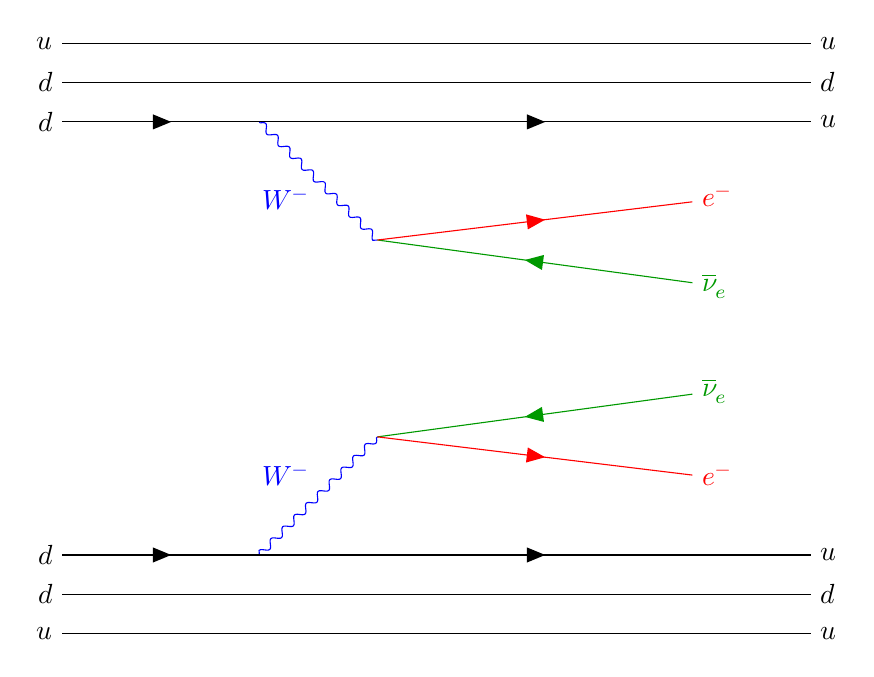
\begin{tikzpicture}
  \begin{feynman}
    \vertex (b);
    \vertex [below=\hei+1cm of b] (c);
    \vertex [below left=\hei and \hei of c] (d);
    \vertex [above left=\hei and \hei of b] (a);
    % spectator quarks vertices
    \vertex [above=\dy of a] (e);
    \vertex [above=\dy of e] (f);
    \vertex [below=\dy of d] (g);
    \vertex [below=\dy of g] (h);
    % external legs
    \vertex [left=\lsx of a] (i1) {$d$};
    \vertex [left=\lsx of d] (i2) {$d$};
    \vertex [right=\ldx of a] (f1) {$u$};
    \vertex [above right=\ange and \lene of b] (f2) {\color{red}$e^-$};
    \vertex [below right=\ange and \lene of b] (f13) {\color{green!60!black}$\overline\nu_e$};
    \vertex [below right=\ange and \lene of c] (f3) {\color{red}$e^-$};
    \vertex [above right=\ange and \lene of c] (f14) {\color{green!60!black}$\overline\nu_e$};
    \vertex [right=\ldx of d] (f4) {$u$};
    % spactator quarks
    \vertex [right=\ldx of e] (f5) {$d$};
    \vertex [left=\lsx of e] (f6) {$d$};
    \vertex [right=\ldx of f] (f7) {$u$};
    \vertex [left=\lsx of f] (f8) {$u$};
    \vertex [right=\ldx of g] (f9) {$d$};
    \vertex [left=\lsx of g] (f10) {$d$};
    \vertex [right=\ldx of h] (f11) {$u$};
    \vertex [left=\lsx of h] (f12) {$u$};

    \diagram* {
      (a) -- [boson, blue, edge label'=$W^-$] (b),
      (c) -- [boson, blue, edge label'=$W^-$] (d),
      (f13) -- [fermion, green!60!black] (b),
      (f14) -- [fermion, green!60!black] (c),
      (i1) -- [fermion] (a),
      (i2) -- [fermion] (d),
      (a) -- [fermion,] (f1),
      (b) -- [fermion, red] (f2),
      (c) -- [fermion, red] (f3),
      (d) -- [fermion] (f4),
      % spectator quarks
      (f6)  -- (e),
      (e)   -- (f5),
      (f8)  -- (f),
      (f)   -- (f7),
      (f10) -- (g),
      (g)   -- (f9),
      (f12) -- (h),
      (h)   -- (f11),

  };
  \end{feynman}
\end{tikzpicture}
\end{document}
